\chapter{L10 -- Modi dominanti, spazio delle fasi ed equivalenza algebrica}

\section{Obiettivo della lezione}

In questa lezione si tirano le fila del lavoro fatto nelle lezioni precedenti su:
\begin{itemize}
    \item evoluzione libera dei sistemi lineari;
    \item forma di Jordan;
    \item modi del sistema;
    \item interpretazione geometrica nello spazio delle fasi.
\end{itemize}

L'idea centrale è la seguente:

\begin{quote}
conoscere gli autovalori e la struttura dei blocchi di Jordan permette di capire \emph{quali andamenti temporali} possono comparire nello stato e, quindi, di capire stabilità, instabilità, velocità di convergenza e dinamica dominante.
\end{quote}

Inoltre, si introduce una seconda idea fondamentale del corso:

\begin{quote}
due sistemi ottenuti l'uno dall'altro mediante un cambio invertibile di coordinate di stato sono \emph{algebricamente equivalenti}: cambiano le coordinate con cui descriviamo lo stato, ma non cambia la sostanza dinamica del sistema.
\end{quote}

\section{Richiamo: evoluzione libera nei casi continuo e discreto}

Per un sistema lineare stazionario a tempo continuo
\[
\dot x(t)=Ax(t)+Bu(t), \qquad x(0)=x_0,
\]
la \emph{evoluzione libera} si ottiene ponendo $u(t)\equiv 0$:
\[
\dot x(t)=Ax(t), \qquad x(0)=x_0,
\]
e vale
\begin{equation}
x(t)=e^{At}x_0.
\label{eq:L10_free_CT}
\end{equation}

Per un sistema lineare stazionario a tempo discreto
\[
x(k+1)=Ax(k)+Bu(k), \qquad x(0)=x_0,
\]
l'evoluzione libera si ottiene ponendo $u(k)\equiv 0$:
\[
x(k+1)=Ax(k), \qquad x(0)=x_0,
\]
e vale
\begin{equation}
x(k)=A^k x_0.
\label{eq:L10_free_DT}
\end{equation}

Queste due formule sono il punto di partenza di tutta l'analisi modale:
\begin{itemize}
    \item nel continuo studiamo $e^{At}$;
    \item nel discreto studiamo $A^k$.
\end{itemize}

Se $A$ è simile a una forma di Jordan $J$, cioè se
\[
A=QJQ^{-1},
\]
allora
\[
e^{At}=Qe^{Jt}Q^{-1},
\qquad
A^k=QJ^kQ^{-1}.
\]
Dunque i \emph{modi temporali} veri e propri compaiono dentro $e^{Jt}$ e $J^k$.

\section{Richiamo sui modi elementari}

Dalle lezioni precedenti sappiamo che:

\begin{itemize}
    \item se $\lambda\in\mathbb{R}$ è un autovalore reale, compaiono modi del tipo
    \[
    e^{\lambda t},\quad te^{\lambda t},\quad t^2 e^{\lambda t},\ \dots
    \qquad \text{(tempo continuo)},
    \]
    e
    \[
    \lambda^k,\quad k\lambda^k,\quad k^2\lambda^k,\ \dots
    \qquad \text{(tempo discreto)};
    \]
    \item se $\lambda=\sigma+j\omega$ è complesso, allora nel continuo compaiono modi del tipo
    \[
    e^{\sigma t}\cos(\omega t), \qquad e^{\sigma t}\sin(\omega t),
    \]
    ed eventualmente anche
    \[
    t e^{\sigma t}\cos(\omega t),\quad
    t e^{\sigma t}\sin(\omega t),\quad
    t^2 e^{\sigma t}\cos(\omega t),\quad
    t^2 e^{\sigma t}\sin(\omega t),\ \dots
    \]
    se il blocco di Jordan associato è di ordine maggiore di $1$;
    \item nel discreto, se $\lambda=\rho e^{j\theta}$, compaiono modi del tipo
    \[
    \rho^k\cos(k\theta),\qquad \rho^k\sin(k\theta),
    \]
    ed eventualmente anche con fattori polinomiali in $k$.
\end{itemize}

\subsection{Interpretazione immediata dei casi reali}

Per $\lambda\in\mathbb{R}$ nel continuo:
\begin{itemize}
    \item se $\lambda<0$, il modo si smorza;
    \item se $\lambda>0$, il modo diverge;
    \item se $\lambda=0$, il modo è critico: può essere costante, oppure polinomialmente divergente se compaiono fattori $t, t^2,\dots$
\end{itemize}

Nel discreto:
\begin{itemize}
    \item se $|\lambda|<1$, il modo converge a zero;
    \item se $|\lambda|>1$, il modo diverge;
    \item se $|\lambda|=1$, il modo è critico.
\end{itemize}

\section{Grafici qualitativi dei modi nel continuo}

I grafici seguenti non servono per fare calcoli numerici, ma per allenare l'intuizione: guardando questi andamenti bisogna imparare a riconoscere subito che tipo di autovalore o di blocco di Jordan c'è dietro.

\subsection{Modi reali non oscillatori}

\begin{figure}[H]
\centering

\begin{subfigure}{0.31\textwidth}
\centering
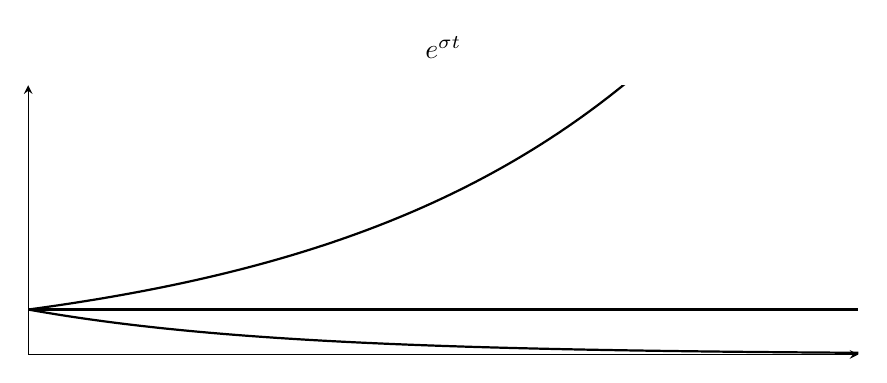
\begin{tikzpicture}
\begin{axis}[
    width=\textwidth,
    height=5cm,
    axis lines=middle,
    xmin=0, xmax=4,
    ymin=0, ymax=6,
    xtick=\empty, ytick=\empty,
    title={$e^{\sigma t}$}
]
\addplot[domain=0:4, samples=200, thick] {1};
\addplot[domain=0:4, samples=200, thick] {exp(x/1.6)};
\addplot[domain=0:4, samples=200, thick] {exp(-x/1.2)};
\end{axis}
\end{tikzpicture}
\caption{Caso base}
\end{subfigure}
\hfill
\begin{subfigure}{0.31\textwidth}
\centering
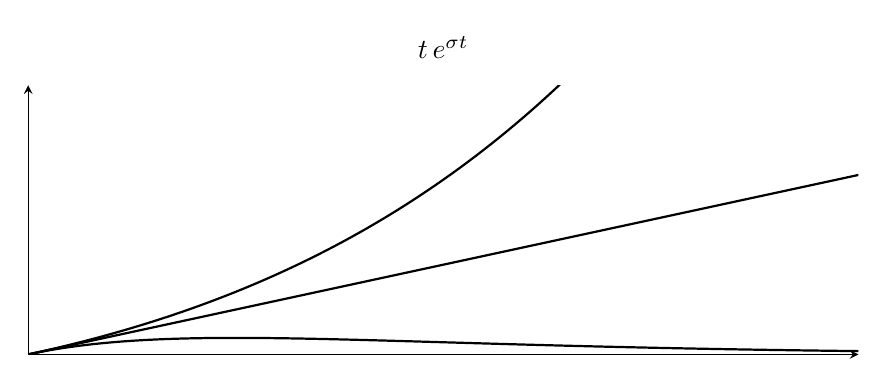
\begin{tikzpicture}
\begin{axis}[
    width=\textwidth,
    height=5cm,
    axis lines=middle,
    xmin=0, xmax=4,
    ymin=0, ymax=6,
    xtick=\empty, ytick=\empty,
    title={$t\,e^{\sigma t}$}
]
\addplot[domain=0:4, samples=200, thick] {x};
\addplot[domain=0:4, samples=200, thick] {x*exp(x/3)};
\addplot[domain=0:4, samples=200, thick] {x*exp(-x)};
\end{axis}
\end{tikzpicture}
\caption{Con fattore lineare}
\end{subfigure}
\hfill
\begin{subfigure}{0.31\textwidth}
\centering
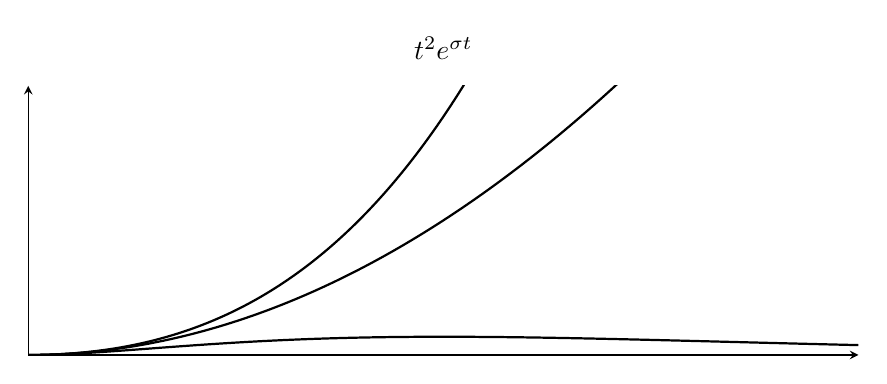
\begin{tikzpicture}
\begin{axis}[
    width=\textwidth,
    height=5cm,
    axis lines=middle,
    xmin=0, xmax=4,
    ymin=0, ymax=8,
    xtick=\empty, ytick=\empty,
    title={$t^2e^{\sigma t}$}
]
\addplot[domain=0:4, samples=200, thick] {x^2};
\addplot[domain=0:4, samples=200, thick] {x^2*exp(x/3.5)};
\addplot[domain=0:4, samples=200, thick] {x^2*exp(-x)};
\end{axis}
\end{tikzpicture}
\caption{Con fattore quadratico}
\end{subfigure}

\caption{Andamenti qualitativi dei modi reali nel continuo: nello stesso grafico si leggono i casi $\sigma=0$, $\sigma>0$ e $\sigma<0$.}
\label{fig:L10_real_modes_CT}
\end{figure}

\paragraph{Lettura della figura.}
\begin{itemize}
    \item La curva costante $1$ corrisponde al caso $\sigma=0$ e blocco di Jordan di ordine $1$.
    \item Le curve $t$ e $t^2$ corrispondono ancora al caso $\sigma=0$, ma con blocchi di Jordan di ordine maggiore.
    \item Le curve crescenti corrispondono a $\sigma>0$.
    \item Le curve che, dopo un transitorio, vanno a zero corrispondono a $\sigma<0$.
\end{itemize}

Un punto molto importante è il seguente:

\begin{quote}
nel continuo, anche se compare un fattore polinomiale $t^r$, se $\sigma<0$ l'esponenziale vince comunque e il modo tende a zero.
\end{quote}

Ad esempio
\[
t e^{-t}\to 0,
\qquad
t^2 e^{-t}\to 0,
\qquad
t^{10}e^{-t}\to 0
\qquad \text{per } t\to +\infty.
\]

\subsection{Modi oscillatori nel continuo}

Se $\lambda=\sigma+j\omega$, i modi reali si ottengono prendendo parte reale e immaginaria di $e^{\lambda t}$, cioè
\[
e^{\sigma t}\cos(\omega t),
\qquad
e^{\sigma t}\sin(\omega t).
\]

Se il blocco di Jordan associato ha ordine maggiore di $1$, compaiono anche
\[
t e^{\sigma t}\cos(\omega t),\qquad
t e^{\sigma t}\sin(\omega t),
\]
oppure
\[
t^2 e^{\sigma t}\cos(\omega t),\qquad
t^2 e^{\sigma t}\sin(\omega t),
\]
e così via.

\begin{figure}[H]
\centering

\begin{subfigure}{0.31\textwidth}
\centering
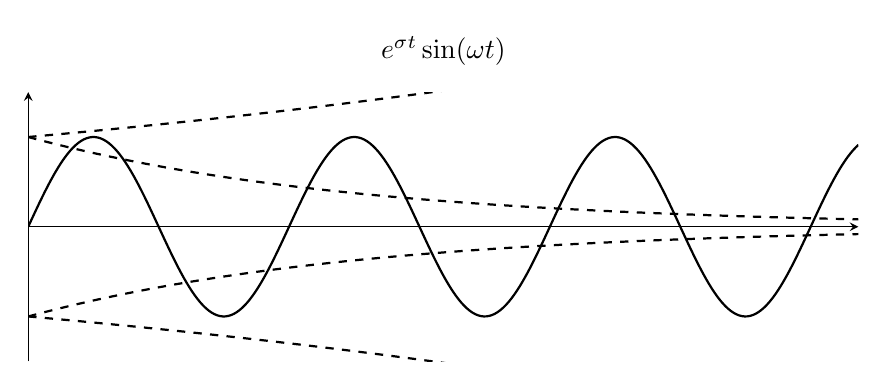
\begin{tikzpicture}
\begin{axis}[
    width=\textwidth,
    height=5cm,
    axis lines=middle,
    xmin=0, xmax=10,
    ymin=-1.5, ymax=1.5,
    xtick=\empty, ytick=\empty,
    title={$e^{\sigma t}\sin(\omega t)$}
]
\addplot[domain=0:10, samples=300, thick] {sin(deg(2*x))};
\addplot[domain=0:10, samples=300, thick, dashed] {exp(-x/4)};
\addplot[domain=0:10, samples=300, thick, dashed] {-exp(-x/4)};
\addplot[domain=0:10, samples=300, thick, dashed] {exp(x/12)};
\addplot[domain=0:10, samples=300, thick, dashed] {-exp(x/12)};
\end{axis}
\end{tikzpicture}
\caption{Ordine $1$}
\end{subfigure}
\hfill
\begin{subfigure}{0.31\textwidth}
\centering
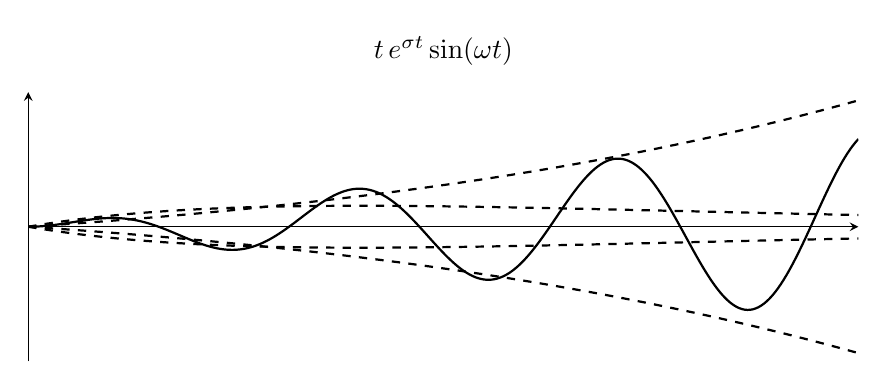
\begin{tikzpicture}
\begin{axis}[
    width=\textwidth,
    height=5cm,
    axis lines=middle,
    xmin=0, xmax=10,
    ymin=-3.5, ymax=3.5,
    xtick=\empty, ytick=\empty,
    title={$t\,e^{\sigma t}\sin(\omega t)$}
]
\addplot[domain=0:10, samples=300, thick] {x*sin(deg(2*x))/4};
\addplot[domain=0:10, samples=300, thick, dashed] {x*exp(-x/4)/2.7};
\addplot[domain=0:10, samples=300, thick, dashed] {-x*exp(-x/4)/2.7};
\addplot[domain=0:10, samples=300, thick, dashed] {x*exp(x/12)/7};
\addplot[domain=0:10, samples=300, thick, dashed] {-x*exp(x/12)/7};
\end{axis}
\end{tikzpicture}
\caption{Ordine $2$}
\end{subfigure}
\hfill
\begin{subfigure}{0.31\textwidth}
\centering
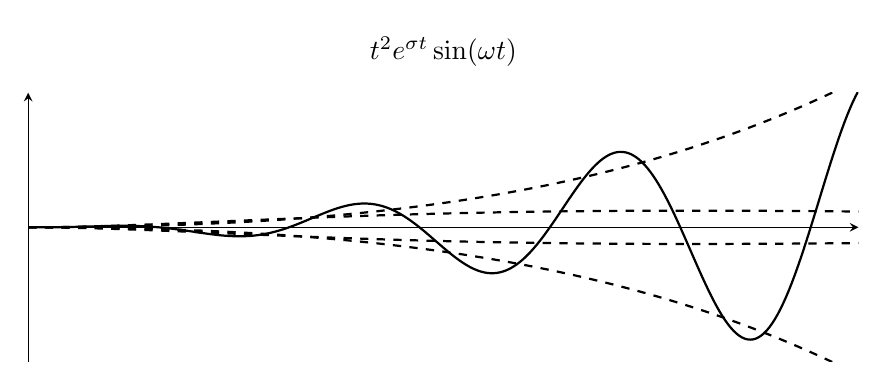
\begin{tikzpicture}
\begin{axis}[
    width=\textwidth,
    height=5cm,
    axis lines=middle,
    xmin=0, xmax=10,
    ymin=-5, ymax=5,
    xtick=\empty, ytick=\empty,
    title={$t^2e^{\sigma t}\sin(\omega t)$}
]
\addplot[domain=0:10, samples=300, thick] {x^2*sin(deg(2*x))/18};
\addplot[domain=0:10, samples=300, thick, dashed] {x^2*exp(-x/4)/14};
\addplot[domain=0:10, samples=300, thick, dashed] {-x^2*exp(-x/4)/14};
\addplot[domain=0:10, samples=300, thick, dashed] {x^2*exp(x/12)/42};
\addplot[domain=0:10, samples=300, thick, dashed] {-x^2*exp(x/12)/42};
\end{axis}
\end{tikzpicture}
\caption{Ordine $3$}
\end{subfigure}

\caption{Modi oscillatori nel continuo. Le linee tratteggiate sono gli inviluppi. Se $\sigma<0$ l'oscillazione è smorzata, se $\sigma=0$ è limitata, se $\sigma>0$ è amplificata.}
\label{fig:L10_complex_modes_CT}
\end{figure}

\paragraph{Osservazione.}
Se $\sigma=0$, l'inviluppo è costante: quindi compaiono oscillazioni non smorzate.
Se invece compaiono fattori $t$, $t^2$, \dots\ anche con $\sigma=0$, l'ampiezza cresce polinomialmente.

\section{Un primo messaggio pratico: i modi permettono di riconoscere il sistema}

Se conosco autovalori e dimensioni dei blocchi di Jordan, allora conosco i modi.
Viceversa, osservando i modi, posso risalire alla struttura spettrale qualitativa del sistema.

Per esempio:
\begin{itemize}
    \item se vedo un termine $e^{-t}$, penso a un autovalore reale negativo;
    \item se vedo un termine $te^{-t}$, penso a un autovalore reale negativo con blocco di Jordan di ordine almeno $2$;
    \item se vedo un termine $e^{-t}\sin t$, penso a una coppia complessa con parte reale negativa;
    \item se vedo un termine $t e^{-t}\sin t$, penso a una coppia complessa con blocco reale di Jordan di ordine almeno $2$;
    \item se vedo un termine costante oppure oscillatorio limitato, penso a un caso critico.
\end{itemize}

Questa capacità di lettura qualitativa è molto importante nella progettazione dei controllori: non interessa solo sapere \emph{quanto vale} un autovalore, ma soprattutto \emph{che andamento induce nel tempo}.

\section{Dominanza modale}

\subsection{Idea intuitiva}

Nella pratica, soprattutto nel controllo, capita spesso che il sistema abbia molti autovalori, ma solo alcuni siano davvero rilevanti per l'andamento a lungo termine.

Il concetto chiave è questo:

\begin{quote}
il modo che decade più lentamente è quello che, a lungo andare, resta visibile; quelli che decadono più velocemente diventano trascurabili.
\end{quote}

Per esempio, nel continuo:
\[
e^{-t}
\qquad \text{e} \qquad
e^{-10t}.
\]
Entrambi vanno a zero, ma $e^{-10t}$ ci va molto più velocemente.  
Infatti
\[
\frac{e^{-10t}}{e^{-t}}=e^{-9t}\to 0.
\]
Quindi, per tempi grandi, il comportamento del sistema è dominato da $e^{-t}$.

\subsection{Polo dominante nel continuo}

Supponiamo di avere autovalori
\[
\lambda_1,\lambda_2,\dots,\lambda_n
\]
e che uno di essi abbia parte reale più grande di tutti:
\[
\Re(\lambda_{\mathrm{dom}})=\max_i \Re(\lambda_i).
\]

Allora, \emph{a meno di cancellazioni dovute alla particolare condizione iniziale}, il comportamento a lungo termine è dominato dai modi associati a $\lambda_{\mathrm{dom}}$.

Se il blocco di Jordan più grande associato a $\lambda_{\mathrm{dom}}$ ha ordine $r$, allora l'andamento dominante sarà del tipo
\begin{equation}
t^{r-1}e^{\lambda_{\mathrm{dom}}t}.
\label{eq:L10_dom_CT}
\end{equation}

\paragraph{Perché compare proprio $t^{r-1}$?}
Perché, per un blocco di Jordan di ordine $r$, i modi associati sono
\[
e^{\lambda t},\quad
t e^{\lambda t},\quad
t^2 e^{\lambda t},\ \dots,\quad
t^{r-1}e^{\lambda t},
\]
e quello con grado polinomiale massimo è il più lento a scomparire rispetto agli altri associati allo stesso autovalore.

\paragraph{Osservazione importante.}
Quando due autovalori hanno parti reali diverse, vince quello con parte reale più grande.
Quando invece hanno la stessa parte reale, allora per capire chi domina bisogna guardare:
\begin{itemize}
    \item il grado del fattore polinomiale;
    \item la presenza di eventuali oscillazioni;
    \item la condizione iniziale.
\end{itemize}

\subsection{Polo dominante nel discreto}

Nel discreto il criterio analogo non è la parte reale, ma il modulo.

Se
\[
|\lambda_{\mathrm{dom}}|=\max_i |\lambda_i|,
\]
allora, a meno di cancellazioni, il comportamento a lungo termine è dominato dai modi associati a $\lambda_{\mathrm{dom}}$.

Se il blocco di Jordan massimo associato ha ordine $r$, allora il modo dominante è del tipo
\begin{equation}
k^{r-1}\lambda_{\mathrm{dom}}^k.
\label{eq:L10_dom_DT}
\end{equation}

Se $\lambda_{\mathrm{dom}}$ è complesso, si avranno oscillazioni moltiplicate da un inviluppo dominato da $|\lambda_{\mathrm{dom}}|^k$.

\subsection{Perché la dominanza modale è importante nel controllo}

Nella progettazione dei controllori spesso si impongono specifiche come:
\begin{itemize}
    \item tempo di assestamento;
    \item sovraelongazione;
    \item rapidità di convergenza;
    \item smorzamento delle oscillazioni.
\end{itemize}

Anche se il sistema a ciclo chiuso può essere di ordine elevato, spesso si cerca di far sì che la dinamica visibile sia dominata da uno o due modi principali, spesso assimilabili a un comportamento del secondo ordine.

Per questo si parla di \textbf{poli dominanti}: sono i poli che determinano la dinamica osservabile a lungo termine.

\section{Un esempio molto semplice di dominanza}

Supponiamo che nel continuo compaiano i due modi
\[
e^{-t}, \qquad e^{-10t}.
\]
Allora
\[
e^{-10t}=e^{-t}e^{-9t},
\]
e il fattore $e^{-9t}$ tende molto rapidamente a zero.

Quindi, per tempi grandi,
\[
c_1e^{-t}+c_2e^{-10t}\approx c_1e^{-t}.
\]

In altre parole:
\begin{quote}
il modo più lento è quello che resta.
\end{quote}

Allo stesso modo, nel discreto, tra
\[
(0.8)^k
\qquad \text{e} \qquad
(0.2)^k
\]
domina $(0.8)^k$, perché
\[
\frac{(0.2)^k}{(0.8)^k}=\left(\frac14\right)^k\to 0.
\]

\section{Spazio delle fasi}

\subsection{Significato geometrico}

Se il sistema ha due variabili di stato, per esempio $x_1$ e $x_2$, allora possiamo rappresentare lo stato come un punto del piano:
\[
x=
\begin{pmatrix}
x_1\\
x_2
\end{pmatrix}.
\]

Lo \textbf{spazio delle fasi} è proprio lo spazio delle variabili di stato.  
Ogni traiettoria del sistema diventa quindi una curva nel piano $(x_1,x_2)$.

Questo è estremamente utile perché ci permette di capire:
\begin{itemize}
    \item se le traiettorie si avvicinano all'origine;
    \item se si allontanano;
    \item se esistono direzioni privilegiate;
    \item se l'equilibrio è stabile, instabile o di tipo sella.
\end{itemize}

\subsection{Sistema omogeneo 2D}

Consideriamo il sistema omogeneo
\[
\dot x = Ax
\]
oppure
\[
x(k+1)=Ax(k).
\]

L'origine $x=0$ è sempre un punto di equilibrio.  
Il tipo di equilibrio dipende dagli autovalori e dagli autovettori (o, più in generale, dalla struttura di Jordan).

\paragraph{Messaggio importante.}
Non basta conoscere solo gli autovalori: per capire \emph{come} si dispongono le traiettorie nel piano, servono anche le direzioni eigenspaziali e quindi, in generale, la struttura completa di $A$.

\subsection{Ritratti di fase qualitativi}

\begin{figure}[H]
\centering

\begin{subfigure}{0.31\textwidth}
\centering
\begin{tikzpicture}[scale=0.9,>=Latex]
\draw[->] (-2.2,0)--(2.2,0) node[right] {$x_1$};
\draw[->] (0,-2.2)--(0,2.2) node[above] {$x_2$};
\fill (0,0) circle (2pt);

\draw[thick,->] (1.8,1.8) .. controls (1,1) and (0.4,0.4) .. (0.08,0.08);
\draw[thick,->] (-1.8,-1.8) .. controls (-1,-1) and (-0.4,-0.4) .. (-0.08,-0.08);
\draw[thick,->] (1.8,-1.5) .. controls (0.8,-1) and (0.3,-0.4) .. (0.06,-0.06);
\draw[thick,->] (-1.6,1.7) .. controls (-0.8,0.9) and (-0.25,0.3) .. (-0.05,0.05);
\end{tikzpicture}
\caption{Nodo stabile}
\end{subfigure}
\hfill
\begin{subfigure}{0.31\textwidth}
\centering
\begin{tikzpicture}[scale=0.9,>=Latex]
\draw[->] (-2.2,0)--(2.2,0) node[right] {$x_1$};
\draw[->] (0,-2.2)--(0,2.2) node[above] {$x_2$};
\fill (0,0) circle (2pt);

\draw[thick,->] (0.08,0.08) .. controls (0.5,0.5) and (1.0,1.0) .. (1.8,1.8);
\draw[thick,->] (-0.08,-0.08) .. controls (-0.5,-0.5) and (-1.0,-1.0) .. (-1.8,-1.8);
\draw[thick,->] (0.06,-0.06) .. controls (0.3,-0.4) and (0.8,-1.0) .. (1.8,-1.5);
\draw[thick,->] (-0.05,0.05) .. controls (-0.25,0.3) and (-0.8,0.9) .. (-1.6,1.7);
\end{tikzpicture}
\caption{Nodo instabile}
\end{subfigure}
\hfill
\begin{subfigure}{0.31\textwidth}
\centering
\begin{tikzpicture}[scale=0.9,>=Latex]
\draw[->] (-2.2,0)--(2.2,0) node[right] {$x_1$};
\draw[->] (0,-2.2)--(0,2.2) node[above] {$x_2$};
\fill (0,0) circle (2pt);

\draw[thick,->] (-1.9,0)--(-0.15,0);
\draw[thick,->] (1.9,0)--(0.15,0);
\draw[thick,->] (0,0.15)--(0,1.9);
\draw[thick,->] (0,-0.15)--(0,-1.9);

\draw[thick,->] (-1.6,1.6) .. controls (-0.7,1.1) and (-0.2,0.5) .. (0,0.18);
\draw[thick,->] (1.6,-1.6) .. controls (0.7,-1.1) and (0.2,-0.5) .. (0,-0.18);

\draw[thick,->] (0,0.18) .. controls (0.2,0.5) and (0.7,1.1) .. (1.6,1.6);
\draw[thick,->] (0,-0.18) .. controls (-0.2,-0.5) and (-0.7,-1.1) .. (-1.6,-1.6);
\end{tikzpicture}
\caption{Sella}
\end{subfigure}

\caption{Ritratti di fase qualitativi per sistemi omogenei bidimensionali.}
\label{fig:L10_phase_portraits}
\end{figure}

\paragraph{Interpretazione.}
\begin{itemize}
    \item Se tutti i modi convergono, l'origine è stabile asintoticamente.
    \item Se tutti i modi divergono, l'origine è instabile.
    \item Se alcuni modi convergono e altri divergono, l'origine è una sella.
\end{itemize}

\section{Equivalenza algebrica tra sistemi lineari stazionari}

\subsection{Definizione}

Consideriamo due sistemi lineari stazionari
\[
\Sigma:
\begin{cases}
x^{+}=Ax+Bu\\
y=Cx+Du
\end{cases}
\qquad
\widetilde{\Sigma}:
\begin{cases}
\tilde x^{+}=\tilde A \tilde x+\tilde B u\\
y=\tilde C \tilde x+\tilde D u
\end{cases}
\]
dove con $x^+$ si intende:
\begin{itemize}
    \item $\dot x$ nel continuo;
    \item $x(k+1)$ nel discreto.
\end{itemize}

I due sistemi si dicono \textbf{algebricamente equivalenti} se esiste una matrice invertibile $T$ tale che
\begin{equation}
x=T\tilde x.
\label{eq:L10_state_change}
\end{equation}

Sostituendo \eqref{eq:L10_state_change} nel sistema originale si ottiene
\[
T\tilde x^{+}=AT\tilde x+Bu
\]
e dunque
\[
\tilde x^{+}=T^{-1}AT\,\tilde x + T^{-1}B\,u.
\]
Inoltre, siccome
\[
y=Cx+Du=CT\tilde x+Du,
\]
si ottiene
\[
y=\tilde C \tilde x+\tilde D u
\]
con
\[
\tilde C=CT,
\qquad
\tilde D=D.
\]

Quindi le relazioni di trasformazione sono:
\begin{equation}
\boxed{
\tilde A=T^{-1}AT,\qquad
\tilde B=T^{-1}B,\qquad
\tilde C=CT,\qquad
\tilde D=D.
}
\label{eq:L10_similarity_system}
\end{equation}

\subsection{Interpretazione}

Questa trasformazione non cambia il sistema in senso fisico o ingresso-uscita: cambia solo il modo in cui descriviamo internamente lo stato.

In altre parole:
\begin{quote}
i due sistemi rappresentano la stessa dinamica, ma in coordinate di stato diverse.
\end{quote}

Per questo motivo:
\begin{itemize}
    \item hanno gli stessi autovalori;
    \item hanno la stessa forma di Jordan a meno dell'ordinamento dei blocchi;
    \item hanno la stessa funzione di trasferimento;
    \item hanno le stesse proprietà strutturali fondamentali.
\end{itemize}

\subsection{Perché questo è importante}

Portare $A$ in forma di Jordan non significa cambiare la sostanza del sistema: significa scegliere coordinate più comode per leggere i modi del sistema.

Perciò tutto quello che abbiamo detto su $J$ vale anche per $A$, semplicemente letto in una base diversa.

\section{Evoluzione libera ed evoluzione forzata}

Fin qui abbiamo ragionato soprattutto sull'evoluzione libera, che dipende solo da $A$:
\[
x(t)=e^{At}x(0),
\qquad
x(k)=A^k x(0).
\]

Ma per il sistema completo l'evoluzione è
\begin{equation}
x(t)=e^{At}x(0)+\int_0^t e^{A(t-\tau)}B\,u(\tau)\,d\tau
\qquad \text{(continuo)},
\label{eq:L10_forced_CT}
\end{equation}
e
\begin{equation}
x(k)=A^k x(0)+\sum_{i=0}^{k-1}A^{k-1-i}B\,u(i)
\qquad \text{(discreto)}.
\label{eq:L10_forced_DT}
\end{equation}

\paragraph{Osservazione concettuale.}
\begin{itemize}
    \item L'evoluzione libera dipende solo da $A$.
    \item L'evoluzione forzata dipende invece sia da $A$ sia da $B$.
\end{itemize}

Questo anticipa il problema della \textbf{raggiungibilità} e della \textbf{controllabilità}:
\begin{quote}
dato un ingresso $u$, quali stati posso raggiungere?
\end{quote}

\subsection{Esempio intuitivo}

Se
\[
B=
\begin{pmatrix}
1\\0\\0\\0
\end{pmatrix},
\]
l'ingresso entra direttamente solo nella prima variabile di stato.

Ma questo non vuol dire che influenzi solo quella: la matrice $A$ può trasferire l'effetto dell'ingresso da una componente dello stato alle altre.

Quindi la capacità di controllare il sistema non dipende solo da dove entra l'ingresso, ma da come \emph{A e B insieme} propagano tale ingresso nello spazio di stato.

\section{Spazio ciclico e struttura dell'evoluzione libera}

L'evoluzione libera
\[
x(t)=e^{At}x(0),
\qquad
x(k)=A^k x(0)
\]
resta confinata nel sottospazio generato dalle potenze di $A$ applicate alla condizione iniziale.

In particolare, nel discreto si introduce il sottospazio ciclico
\[
S_{x_0}=\operatorname{span}\{x_0,Ax_0,A^2x_0,\dots,A^{p-1}x_0\},
\]
dove $p=\dim S_{x_0}$.

Nel continuo il senso geometrico è lo stesso: l'evoluzione libera resta nel sottospazio $A$-invariante generato da $x_0$.

Questo è coerente con l'analisi modale:
\begin{itemize}
    \item se $x_0$ eccita certi modi, essi compaiono nella traiettoria;
    \item se $x_0$ non ha componente lungo un certo sottospazio modale, quel modo può non comparire.
\end{itemize}

\section{Riepilogo finale sugli andamenti nel tempo}

Possiamo riassumere gli andamenti possibili nel modo seguente.

\subsection*{Tempo continuo}

\begin{itemize}
    \item Se $\lambda_i\in\mathbb{R}$, i modi associati sono
    \[
    e^{\lambda_i t},\quad
    t e^{\lambda_i t},\quad
    \dots,\quad
    t^{p_i-1}e^{\lambda_i t},
    \]
    dove $p_i$ è la dimensione del blocco di Jordan più grande associato a $\lambda_i$.
    \item Se $\lambda_i=\sigma_i+j\omega_i\in\mathbb{C}$, i modi reali associati sono
    \[
    e^{\sigma_i t}\cos(\omega_i t),\quad
    e^{\sigma_i t}\sin(\omega_i t),
    \]
    ed eventualmente anche con fattori $t, t^2,\dots$
\end{itemize}

\subsection*{Tempo discreto}

\begin{itemize}
    \item Se $\lambda_i\in\mathbb{R}$, i modi associati sono
    \[
    \lambda_i^k,\quad
    k\lambda_i^k,\quad
    \dots,\quad
    k^{p_i-1}\lambda_i^k.
    \]
    \item Se $\lambda_i=\rho_i e^{j\theta_i}\in\mathbb{C}$, i modi reali associati sono
    \[
    \rho_i^k\cos(k\theta_i),\quad
    \rho_i^k\sin(k\theta_i),
    \]
    eventualmente moltiplicati per $k, k^2,\dots$
\end{itemize}

\section{Messaggio conclusivo della lezione}

Questa lezione si può sintetizzare così:

\begin{enumerate}
    \item l'evoluzione libera di un sistema lineare è governata da $e^{At}$ oppure da $A^k$;
    \item gli andamenti temporali si leggono dai blocchi di Jordan;
    \item il comportamento a lungo termine è determinato dai \textbf{modi dominanti};
    \item due sistemi simili sono algebricamente equivalenti, cioè descrivono la stessa dinamica in coordinate diverse;
    \item quando si passa all'evoluzione forzata entra in gioco anche $B$, e questo apre naturalmente ai concetti di raggiungibilità e controllabilità.
\end{enumerate}

In particolare, per l'analisi qualitativa, bisogna abituarsi a pensare così:
\[
\text{autovalori} + \text{blocchi di Jordan}
\quad \Longrightarrow \quad
\text{modi}
\quad \Longrightarrow \quad
\text{stabilità, rapidità, oscillazioni, dominanza}.
\]

Questo è il vero ponte tra algebra lineare e comportamento dinamico dei sistemi.